\documentclass[11pt]{article}

\usepackage{centernot}
\usepackage{amssymb}
\usepackage{xcolor}
\definecolor{myblue}{RGB}{0, 0, 255} 
\definecolor{mygreen}{RGB}{0, 180, 80}
\definecolor{myred}{RGB}{153, 0, 0}
\definecolor{myorange}{RGB}{255, 153, 51}
\definecolor{mypurple}{RGB}{102, 0, 204}
\usepackage{verbatim}
\usepackage{multicol}
\usepackage{enumitem}
\usepackage{amsfonts}
\usepackage{amsmath}
\usepackage[utf8]{inputenc}
\usepackage[export]{adjustbox}  % for correct logo rendering
\usepackage{fancyhdr}  % for header/footer formatting
\usepackage{hyperref}  % for hyper-references
\usepackage{datetime}  % to update month in footer
\usepackage{array}  % more flexible tables
\usepackage[includeheadfoot,
            left=1in,
            right=1in,
            top=0.75in,
            bottom=0.75in,
            headheight=40pt]{geometry} % geometry needs to know headheight to correctly render the footer
\usepackage{tikz} % For drawing grid boxes

\definecolor{darkblue}{RGB}{0, 0, 139}
\definecolor{lightblue}{RGB}{173, 216, 230}

% desired format for footer
\newdateformat{monthyeardate}{%
  \monthname[\THEMONTH] \THEYEAR}

% set up header/footer
\pagestyle{fancy}
\fancyhf{}  % clear all headers/footers
\renewcommand{\headrulewidth}{0pt}  % remove header rule
\renewcommand{\footrulewidth}{0pt}  % remove footer rule

% set up header

\fancypagestyle{firstpage}{
    \fancyhead[L]{
    \vspace{0pt}
    \hspace{-8pt}
    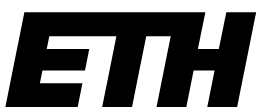
\includegraphics[width=0.1\textwidth]{docimgs/eth_logo_kurz_pos.png}\\
    \textbf{Swiss Federal Institute of Technology}\\
    \textbf{Zurich}\\
    %\textbf{ } \\
    
    }    

    \fancyhead[R]{
    \raggedleft
    %\vspace{20pt}
    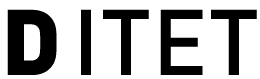
\includegraphics[width=0.13\textwidth]{docimgs/eth_ditet_logo_pos.png}\\
     \textbf{Dept. of Information Technology and} \\ \textbf{Electrical Engineering}  \\
     %\textbf{Chair for Mathematical Information} \\ \textbf{Information Science} \\

    }
}

% set up footer
\fancyfoot[L]{mdietz, ÜS 10}
\fancyfoot[C]{\thepage}
\fancyfoot[R]{\monthyeardate\today}

% set up section/subsection titles
\renewcommand{\thesection}{\arabic{section}}
\renewcommand{\thesubsection}{\arabic{subsection}}

% command used for simply emphasizing suggestions
\newcommand{\suggestion}[1]{{\itshape #1}}

%--- commands for transform arrows----------------
\newcommand{\transform}[2]{%
    \begin{tikzpicture}
        % Open circle
        \draw[thick] (0,0) circle (0.1);
        % Line with number above and adjustable length
        \draw[thick] (0.1,0) -- (#2,0) node[midway, above] {#1};
        % Filled circle
        \filldraw[thick] (#2,0) circle (0.1);
    \end{tikzpicture}%
}
\newcommand{\invtransform}[2]{%
    \begin{tikzpicture}
        % filled circle
        \filldraw[thick] (0,0) circle (0.1);
        % Line with number above and adjustable length
        \draw[thick] (0.1,0) -- (#2 -0.1,0) node[midway, above] {#1};
        % open circle
        \draw[thick] (#2,0) circle (0.1);
    \end{tikzpicture}%
}
\newcommand{\verticaltransform}[4]{%
    \begin{tikzpicture}
        % Open circle at the bottom with text below
        \filldraw[thick] (0,0) circle (0.1) node[below=3pt] {$#4$};
        % Vertical line with number on the left
        \draw[thick] (0,0.1) -- (0,#2 -0.1) node[midway, left] {#1};
        % Filled circle at the top with text above
        \draw[thick] (0,#2) circle (0.1) node[above=3pt] {$#3$};
    \end{tikzpicture}%
}
\newcommand{\verticalinvtransform}[4]{%
    \begin{tikzpicture}
        % Open circle at the bottom with text below
        \draw[thick] (0,0) circle (0.1) node[below=3pt] {$#4$};
        % Vertical line with number on the left
        \draw[thick] (0,0.1) -- (0,#2) node[midway, left] {#1};
        % Filled circle at the top with text above
        \filldraw[thick] (0,#2) circle (0.1) node[above=3pt] {$#3$};
    \end{tikzpicture}%
}

\begin{document}
\thispagestyle{firstpage}

\setlength{\headheight}{1 \baselineskip}  % accomodate header
\setlength{\parindent}{0pt}  % remove initial paragraph indent
\setlength{\parskip}{\baselineskip}  % add skip between paragraphs

\vspace*{-5px}
\section*{Übungsstunde 10}

\section*{Themenüberblick}
\begin{itemize}
    \item \textbf{$\mathcal{Z}$-Transformation}
    \item[] Definition, Konvergenzgebiete und Eigenschaften der $\mathcal{Z}$-Transformation
    \item[] Zusammenhang zwischen $\mathcal{Z}$-Transformation, Laplace Transformation und DTFT
    \item[] Anwendungen der $\mathcal{Z}$-Transformation auf zeitdiskrete LTI-Systeme
\end{itemize}

\section*{Aufgaben für diese Woche}
\vspace{-0.5cm}

\textbf{114}, \textbf{115}, 116 117 118, \textbf{119}, \textbf{120}, 121, \textbf{122}\\
\vspace{-0.5cm}

Die \textbf{fettgedruckten} Übungen empfehle ich, weil sie wesentlich zu eurem Verständnis der Theorie beitragen und/oder sehr prüfungsrelevant sind.

\vfill \null
\pagebreak

\section*{$\mathcal{Z}$-Transformation}
\vspace*{-0.5cm}
\subsection*{Definition}
\vspace*{-0.5cm}
\fcolorbox{darkblue}{lightblue}{%
    \parbox{\dimexpr\linewidth-2\fboxsep-2\fboxrule\relax}{
    \vspace*{0.15cm}
    $$\mathcal{Z}\{x[n]\} = X(z) = \sum_{n=-\infty}^\infty x[n]z^{-n}, \hspace{20pt} z \in \mathbb{C}$$
}}%

Es kann sein, dass die Summe $\sum_{n=-\infty}^\infty x[n]z^{-n}$ möglicherweise nicht konvergiert. Deswegen ist die $\mathcal{Z}$-Transformation nur im Konvergenzgebiet definiert.

\subsection*{Konvergenzgebiet, Region of Convergence (\textit{ROC})}
\vspace*{-0.5cm}
\fcolorbox{darkblue}{lightblue}{%
    \parbox{\dimexpr\linewidth-2\fboxsep-2\fboxrule\relax}{
    \vspace*{0.15cm}
    $$\text{ROC}_X = \{z \in \mathbb{C} \; : \; X(z) \text{ konvergiert absolut}\}$$
}}%
\begin{itemize}[leftmargin = 0pt]
    \item[] Es sei $z= re^{2\pi i \theta}$, somit $\displaystyle\sum_{n=-\infty}^\infty \left| x[n]r^{-n}e^{-2\pi i n \theta} \right| = \displaystyle\sum_{n=-\infty}^\infty \left| x[n]r^{-n} \right|$
    \item[] $\implies$ ROC hängt nur von $|z|=r$ ab.
    \item[] $\implies$ ROC besteht aus Kreisscheiben zentriert um den Ursprung. Also hat ROC$_X$ die Form:
    $$\text{ROC}_X = \{x \in \mathbb{C} \; : \; 0 \leq R_- < |z| < R_+ \leq \infty\}$$
    \item[] Somit folgt, dass das Konvergenzgebiet \textbf{zusammenhängend} sein muss.
    \item[] Wenn die $\mathcal{Z}$-Transformation $X(z)$ von $x[n]$ rational ist, dann enthält die ROC keine Pole, sondern die ROC ist durch die Pole beschränkt oder das Konvergenzgebiet geht ins Unendliche. Diese Eigenschaft ist eine triviale Konsequenz vom Fakt, dass $X(z)$ bei einem Pol gegen unendlich geht und somit nicht konvergiert.
    \item[] Wir unterscheiden bezüglich des Konvergenzgebietes zwischen vier verschiedenen Fällen:
    \begin{enumerate}
        \item \textbf{Rechtsseitiges Signal}
        \item[] \begin{center}
            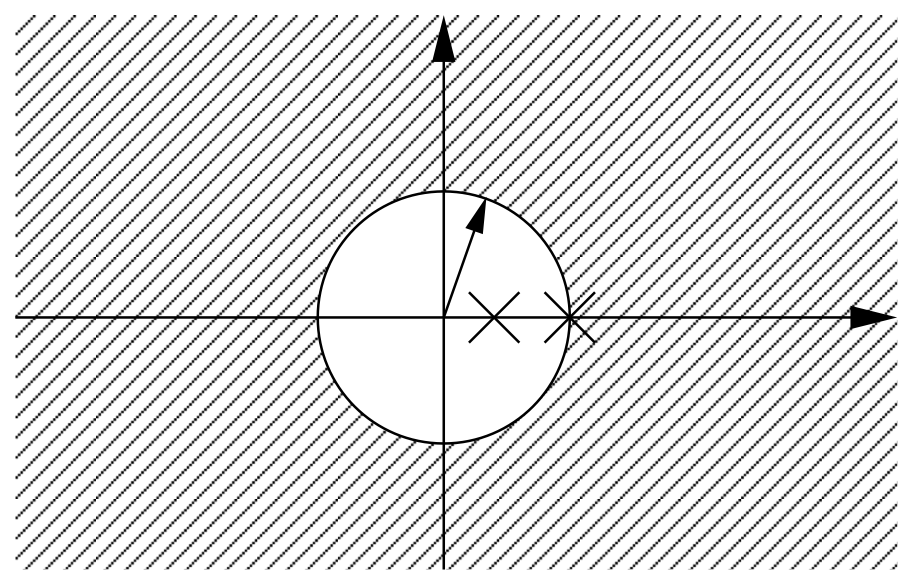
\includegraphics[width=0.4\linewidth]{docimgs/Rechtsseitig.png}
        \end{center}
        \item[] Wenn $x[n]$ ein rechtsseitiges Signal ist und der Kreis $|z|=r_0$ in der ROC ist, dann sind alle $z$ mit $|z|>r_0$ ebenfalls in der ROC.
        $$X(z) = \sum_{n=N_1}^\infty x[n]z^{-n}$$
        \item[] Ein rechtsseitiges Signal ist immer null vor einem gewissen Wert von $n=N_1$. Wenn nun der Kreis $|z|=r_0$ in der ROC liegt, dann ist $x(n)r_0^{-n}$ absolut summierbar. Wenn wir nun $|z|=r_1 > r_0$ betrachten, dann zerfällt $r_1^{-n}$ schneller als $r_0^{-n}$ für steigende $n$. Also ist $x(n)r_1^{-n}$ ebenfalls absolut summierbar. $z = \infty$ kann aber muss nicht in der ROC enthalten sein.
        \item[] \begin{itemize}
            \item $N_1 < 0$: Die Summe enthält Terme von $z$ mit positiven Exponenten, welche unbeschränkt werden für $|z| \to \infty$. Deshalb enthält die ROC eines rechtsseitigen Signales im Allgemeinen nicht $|z|=\infty$.
            \item $N_1 \geq 0$: Für kausale Signale hingegen, d.h. für Sequenzen, die null sind für $n<0$, ist $N_1$ positiv, somit beinhaltet die ROC $|z|=\infty$.
        \end{itemize}
        \item[] Wenn die $\mathcal{Z}$-Transformation $X(z)$ von $x[n]$ rational ist und $x[n]$ rechtsseitig ist, dann ist die ROC die Region in der komplexen Ebene \textbf{ausserhalb des betragsweise grössten Poles} von $X(z)$ (möglicherweise inklusive $|z|=\infty$).
        
        \item \textbf{Linksseitiges Signal}
        \item[] \begin{center}
            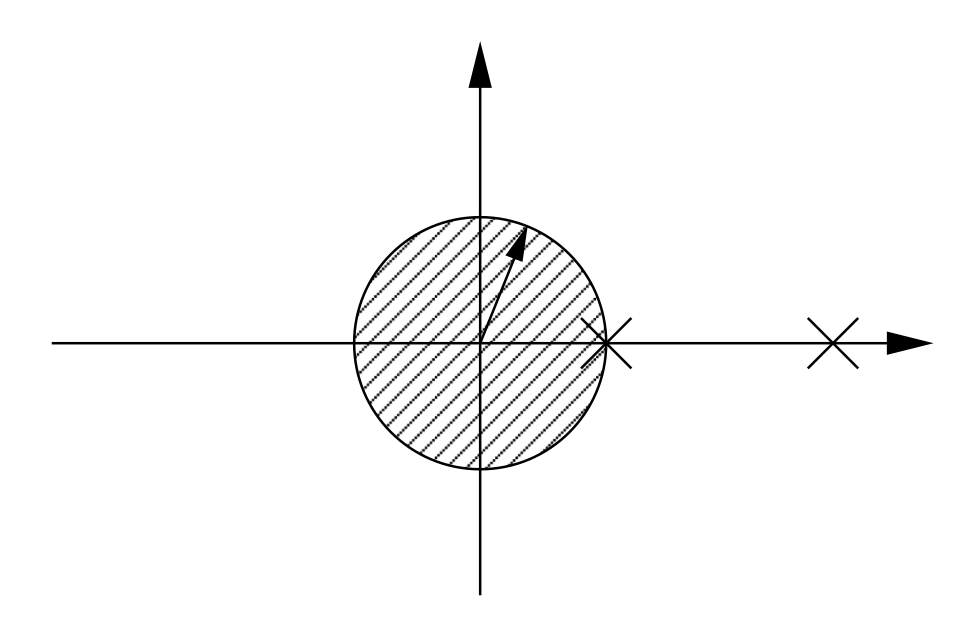
\includegraphics[width=0.4\linewidth]{docimgs/Linksseitig.png}
        \end{center}
        \item[] Wenn $x[n]$ ein linksseitiges Signal ist und wenn der Kreis $|z| = r_0$ in der ROC liegt, dann liegen alle $z$ mit $0 < |z| < r_0$ ebenfalls in der ROC. 
        $$X(z) = \sum_{k=-\infty}^M x[n]z^{-n}$$
        \item[] Die Argumentation ist analog zu rechtsseitigen Signalen. $z=0$ kann aber muss nicht in der ROC enthalten sein.
        \item[] \begin{itemize}
            \item $M > 0$: $X(z)$ enthält negative Exponenten von $z$, welche unbeschränkt werden für $|z|\to 0$. Deshalb enthalten linksseitige Signale im Allgemeinen nicht $z=0$.
            \item $M \leq 0$: In diesem Fall enthält die ROC $z=0$.
        \end{itemize}
        \item[] Wenn die $\mathcal{Z}$-Transformation $X(z)$ von $x[n]$ rational ist und $x[n]$ linksseitig ist, dann ist die ROC die Region in der komplexen Ebene \textbf{innerhalb des betragsweise kleinsten Poles} von $X(z)$ (ausser wie bereits gesagt möglicherweise $z=0$).
        
        \item \textbf{Beidseitiges Signal}
        \item[] \begin{center}
            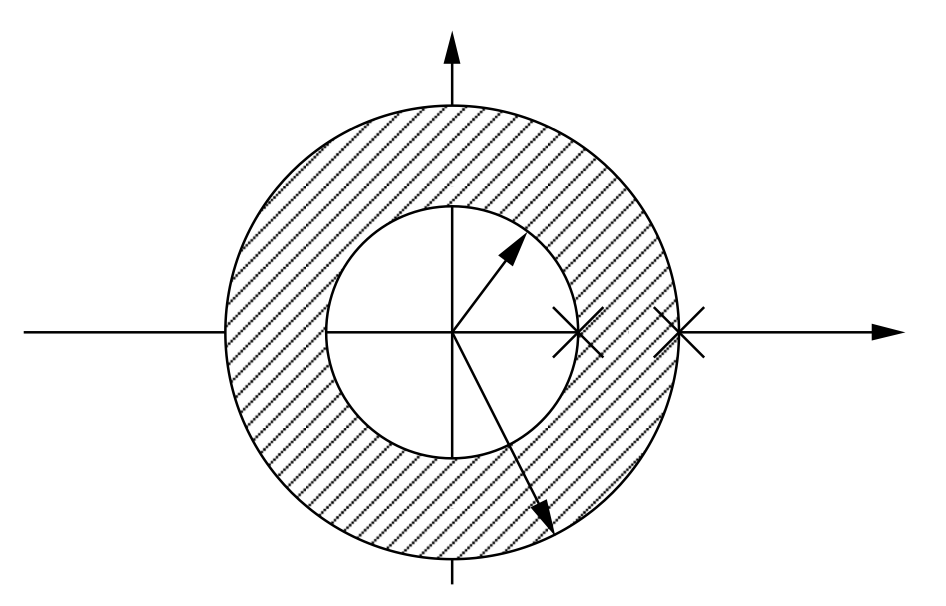
\includegraphics[width=0.35\linewidth]{docimgs/Beidseitig.png}
        \end{center}
        \item[] Ein beidseitiges Signal kann als Summe von einem rechtsseitigen und einem linksseitigen Signal geschrieben werden. Diese Summe konvergiert dort, wo beide Komponenten kovergieren. Somit enthält die ROC die Schnittmenge der ROCs vom rechtsseitigen und linksseitigen Signal.
        
        \item \textbf{Signale endlicher Länge}
        \item[] Ein Signal endlicher Länge nimmt nur an einer endlichen Anzahl an Stellen Werte ungleich null an, also z.B. für $n$ mit $ -\infty < N \leq n \leq M <\infty $. Also ist die $\mathcal{Z}$-Transformation die Summe einer endlichen Anzahl Terme und muss somit für $z\neq 0, \infty $ konvergieren, weil dann jeder Term der Summe endlich ist. Die ROC kann aber muss nicht $z=0$ oder $\infty$ enthalten.
    \end{enumerate}
\end{itemize}

\vspace*{-0.25cm}
\subsection*{Eigenschaften der $\mathcal{Z}$-Transformation}
\vspace*{-0.5cm}
\begin{itemize}
    \item \textbf{Linearität}:
        $$\mathcal{Z}\{ax[n] + by[n]\} = aX(z) + bY(z)$$
    \item[] Das Konvergenzgebiet ist mindestens ROC$_X \cap $ ROC$_Y$
    \item \textbf{Zeitverschiebung}:
        $$\mathcal{Z}\{x[n-n_0]\} = z^{-n_0}X(z)$$
    \item[] Das Konvergenzgebiet bleibt gleich.
    \item \textbf{Faltung}:
        $$y[n] = (x \ast h)[n] \hspace{8pt} \transform{$\mathcal{Z}$}{1} \hspace{8pt} Y(z) = X(z)H(z) $$
    \item[] Das Konvergenzgebiet ist mindestens ROC$_X \cap $ ROC$_Y$
    \item \textbf{Umkehrformel}:
        $$x[n] = \frac{1}{2 \pi i} \oint_C X(z)z^{n-1} \text{d}z$$
    \item[] $C$ ist ein kreisförmiger Pfad im Gegenuhrzeigersinn in der ROC. Diese Umkehrformel sagt gemäss Residuumssatz (aus KomA) nichts anderes aus als dass $x[n] = \sum$ (Residuen an den Polen von $X(z)z^{n-1}$ ausgewertet).
    \item[] Dieses Integral muss man in SST1 jedoch sozusagen nie berechnen, man muss in den allermeisten Fällen die Transformationstabellen in der Formelsammlung verwenden.
\end{itemize}

\pagebreak

\subsection*{Aufgabe 115}
\vspace*{-0.5cm}
In den folgenden Pol-Nullstellen Diagrammen sind die ROCs in grau schraffiert und der Einheitskreis in Rot dargestellt.
\vspace*{-0.5cm}
\begin{itemize}
    \item[a)] Gibt es eine $\mathcal{Z}$-Transformierte mit einer solchen ROC?
    \item[b)] Betrachten Sie das Pol-Nullstellendiagramm der $\mathcal{Z}$-Transformierten $X(z)$. Das zugrundeliegende Signal $x[n]$ ist gegeben durch eine Summe von Exponentialfunktionen. Welche Pole entsprechen linksseitigen und welche rechtsseitigen Exponentialfunktionen?
    \item[c)] Charakterisieren Sie die möglichen zugehörigen ROCs dieses Pol-Nullstellen Diagramms.
    \item[d)] Gibt es eine $\mathcal{Z}$-Transformierte, die den folgenden Pol-Nullstellen Diagrammen mit eingezeichneter ROC entsprechen?
\end{itemize}
\vspace*{-0.5cm}
\noindent
\begin{minipage}[t]{0.25\textwidth}
    a)\\
    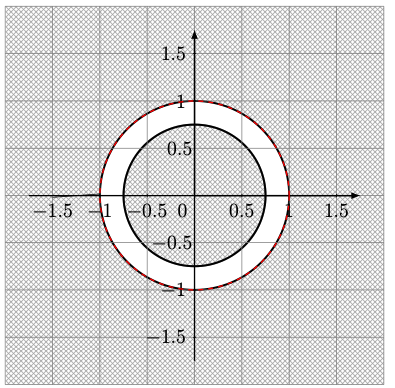
\includegraphics[width=\linewidth]{docimgs/a.png}
\end{minipage}
\hfill
\begin{minipage}[t]{0.25\textwidth}
    b)\\
    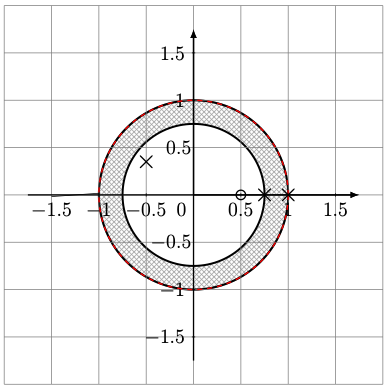
\includegraphics[width=\linewidth]{docimgs/b.png}
\end{minipage}
\hfill
\begin{minipage}[t]{0.25\textwidth}
    c)\\
    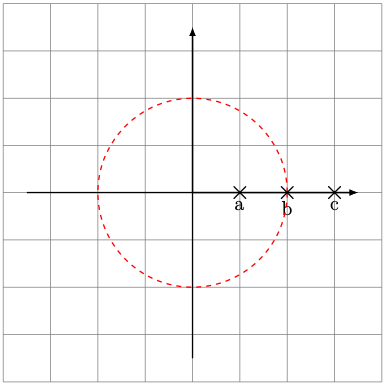
\includegraphics[width=\linewidth]{docimgs/c.png}
\end{minipage}

\noindent
\begin{minipage}[t]{0.25\textwidth}
    d.i)\\
    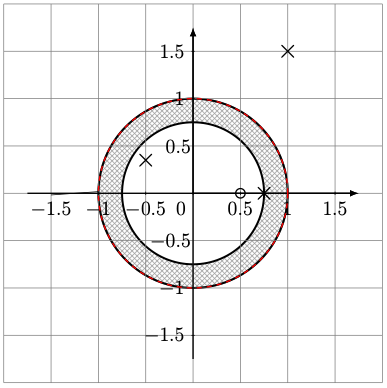
\includegraphics[width=\linewidth]{docimgs/di.png}
\end{minipage}
\hfill
\begin{minipage}[t]{0.25\textwidth}
    d.ii)\\
    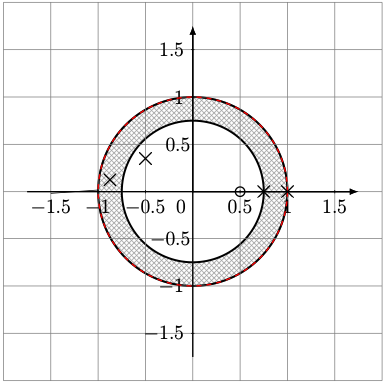
\includegraphics[width=\linewidth]{docimgs/dii.png}
\end{minipage}
\hfill
\begin{minipage}[t]{0.25\textwidth}
    d.iii)\\
    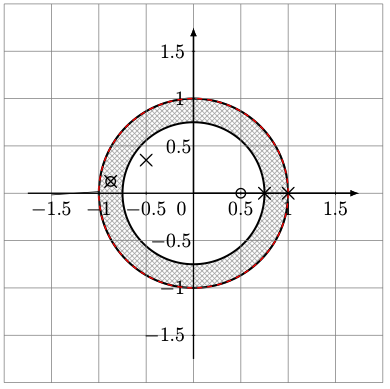
\includegraphics[width=\linewidth]{docimgs/diii.png}
\end{minipage}


\begin{tikzpicture}
    % Define the box size and grid spacing
    \draw[step=0.5cm,gray!50,very thin] (0,0) grid (16.5,4.5
    ); % (0,0) is bottom-left corner, (10,10) is top-right corner
\end{tikzpicture}

\pagebreak

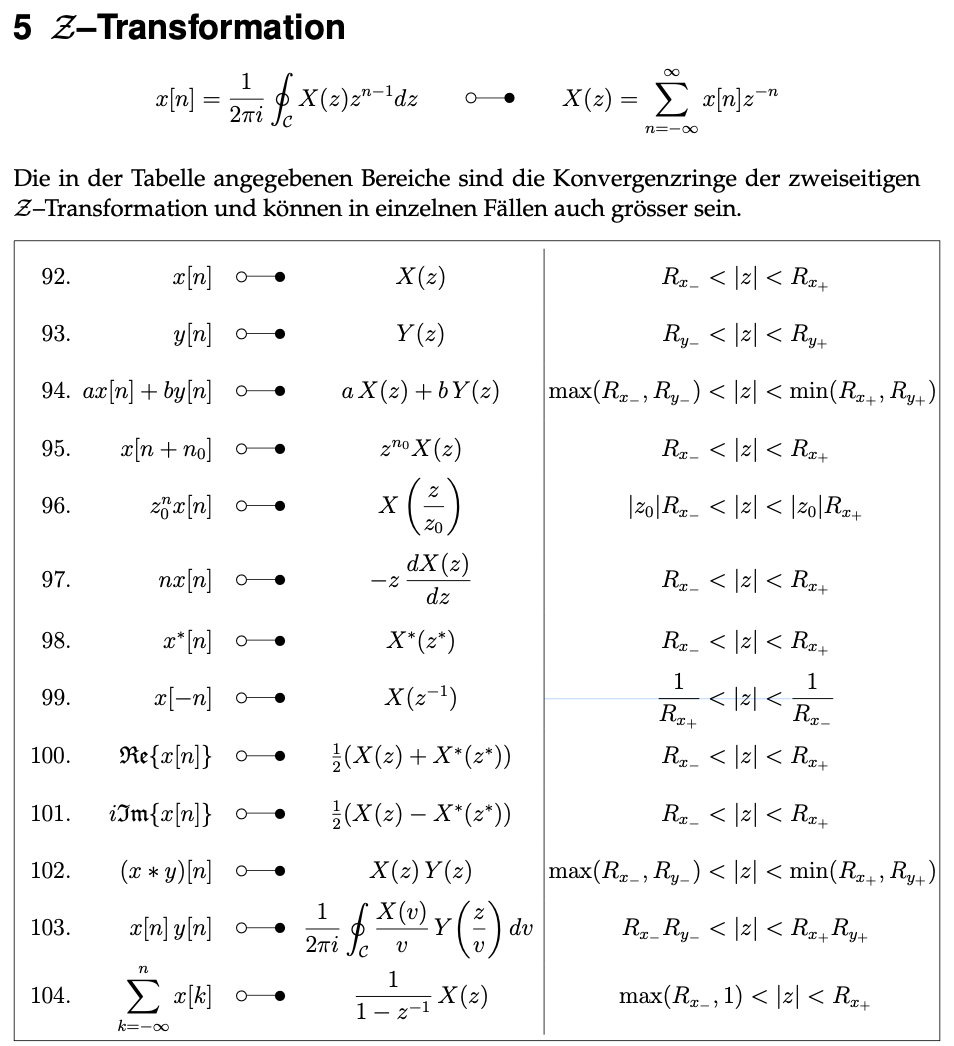
\includegraphics[width=\linewidth]{docimgs/Z-Transformation.png}

\vfill \null
\pagebreak

\begin{center}
    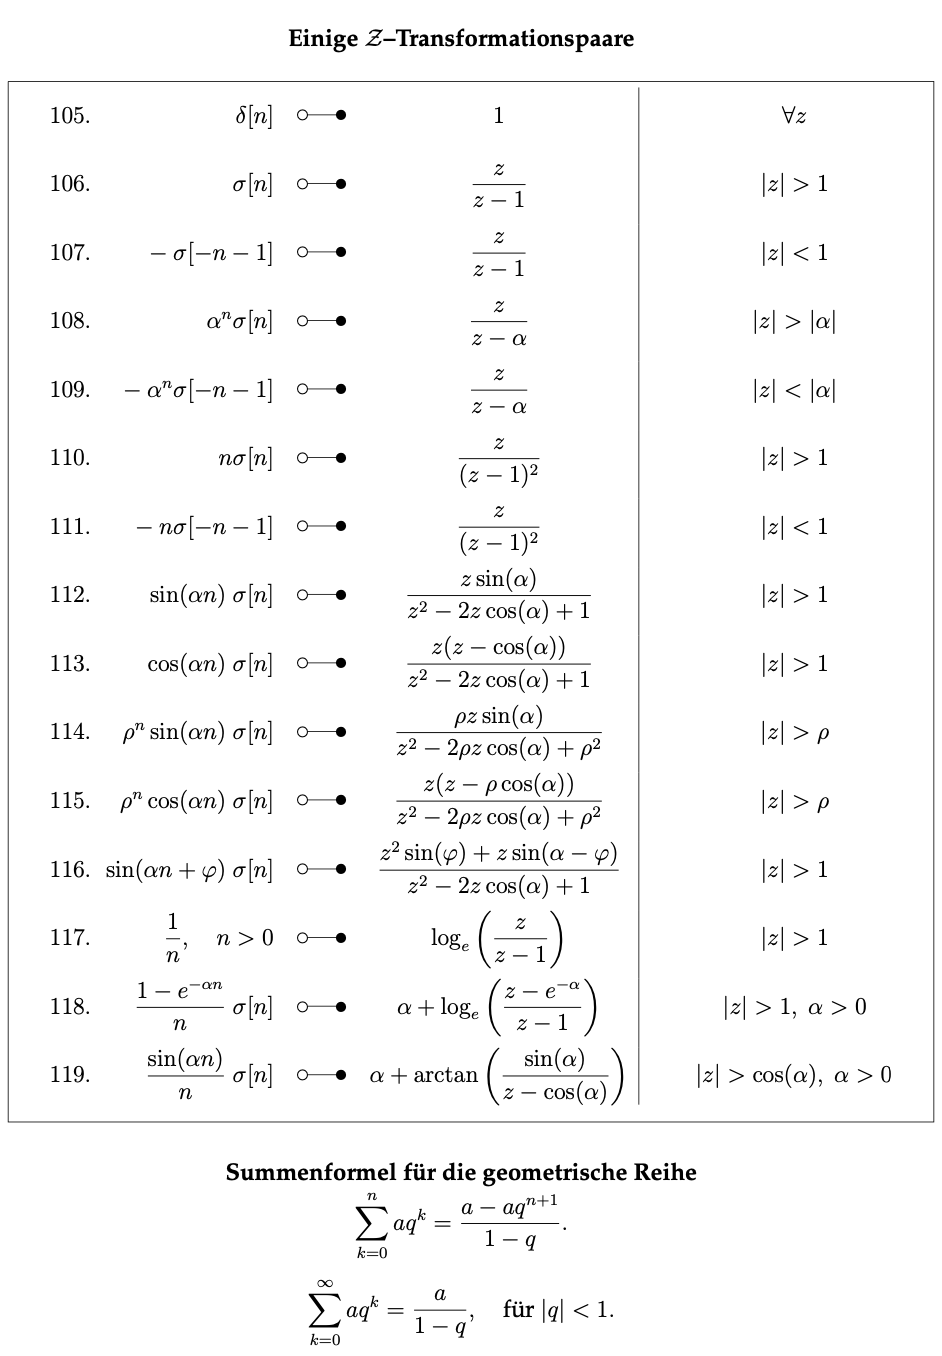
\includegraphics[width=0.9\linewidth]{docimgs/Z-Transformationspaare.png}
\end{center}

\pagebreak

\subsection*{Zusammenhang zwischen $\mathcal{Z}$-Transformation und Laplace Transformation}
\vspace*{-1cm}
\noindent
\begin{minipage}[t]{0.45\textwidth}
    $$(\textbf{$\mathcal{Z}$-Transf.:}) \hspace{20pt} X(z) = \sum_{n=-\infty}^\infty x[n] z^{-n}$$
\end{minipage}
\hfill
\begin{minipage}[t]{0.45\textwidth}
    $$(\textbf{Laplace:}) \hspace{20pt} X(s) = \int_{-\infty}^\infty x(t) e^{-st} \text{d}t$$
\end{minipage}

Die $\mathcal{Z}$-Transformation ist das zeitdiskrete Analogon zur Laplace-Transformation. Die Beziehung zwischen $\mathcal{Z}$-Transformation und Laplace-Transformation kann man verstehen wie die Beziehung zwischen DTFT und der zeitkontinuierlichen Fouriertransformation.

\vspace*{-0.5cm}
\subsection*{Zusammenhang zwischen $\mathcal{Z}$-Transformation und DTFT}
\vspace*{-1cm}
\noindent
\begin{minipage}[t]{0.45\textwidth}
    $$(\textbf{$\mathcal{Z}$-Transf.:}) \hspace{20pt} X(z) = \sum_{n=-\infty}^\infty x[n] z^{-n}$$
\end{minipage}
\hfill
\begin{minipage}[t]{0.45\textwidth}
    $$(\textbf{DTFT:}) \hspace{20pt} \hat{x}(\theta) = \sum_{n=-\infty}^\infty x[n] e^{-2 \pi i n \theta}$$
\end{minipage}

Wenn wir nun die Definition der $\mathcal{Z}$-Transformation mit der DTFT formal vergleichen, dann sehen wir, dass die DTFT nichts anderes ist als die $\mathcal{Z}$-Transformation für $z=e^{2\pi i \theta}$. Das heisst, die DTFT ist ein Spezialfall der $\mathcal{Z}$-Transformation, nämlich die $\mathcal{Z}$-Transformation \textbf{ausgewertet auf dem Einheitskreis} in der komplexen Ebene.

Die Multiplikation von $x[n]$ (dem Wert des Signals im Zeitbereich zum Zeitpunkt $n$) mit $e^{-2 \pi i n \theta}$ kann interpretiert werden als eine \textbf{Rotation} von $x[n]$ in der komplexen Ebene um einen Winkel von $-2 \pi i n \theta$. Das Vorzeichen ist eine Konvention und kommt aus dem negativen Exponenten der DTFT Formel.

Die DTFT summiert nun die Beiträge des Signals zu allen Zeitpunkten, $-\infty < n < \infty$, nach diesen Rotationen. Diese Aufsummierung misst im Grunde wie viel der Frequenz $\omega = 2 \pi \theta$ im Signal $x[n]$ präsent ist.

\vspace*{-0.5cm}
\subsubsection*{Wieso der Einheitskreis?}
\vspace*{-0.5cm}
In der DTFT beschränken wir $z = e^{2 \pi i \theta}$ auf den Einheitskreis, denn die DTFT analysiert ein Signal auf rein \textbf{oszillatorisches Verhalten}. Punkte auf dem Einheitskreis entsprechen \textbf{komplexen Sinuswellen verschiedener Frequenzen}. Indem die DTFT die Beiträge von $x[n]e^{-2 \pi i n \theta}$ summiert, "projiziert" sie $x[n]$ auf diese Sinuswellen, um zu bestimmen, wie stark $x[n]$ bei jeder Frequenz schwingt. So findet man die "Frequenzbestandteile" eines Signals $x[n]$ (wie wenn man z.B. einen Ton in einzelne Noten zerlegt).

\vspace*{-0.5cm}
\subsubsection*{Unterschied zur $\mathcal{Z}$-Transformation}
\vspace*{-0.5cm}
In der $\mathcal{Z}$-Transformation erlaubt $z= r e^{2 \pi i \theta}$ eine Analyse ausserhalb des Einheitskreises, indem eine radiale Komponente $r$ eingeführt wird. Diese Magnitude $r$  ermöglicht es uns, das Verhalten des Signals zu untersuchen:
\vspace*{-0.5cm}
\begin{itemize}
    \item Wenn es gedämpft ist ($|z|<1$), wie bei Signalen, die im Laufe der Zeit abklingen.
    \item Wenn es verstärkt wird ($|z|>1$), wie bei wachsenden Signalen.
\end{itemize}

\vspace*{-0.5cm}
\subsubsection*{Warum brauchen wir sowohl $\mathcal{Z}$-Transformation als auch DTFT?}
\vspace*{-0.5cm}
Die DTFT eignet sich für die Analyse im Frequenzbereich, ist jedoch auf den Einheitskreis beschränkt. Sie konzentriert sich auf das Verständnis von Signalen im Hinblick auf ihren Frequenzinhalt, was ideal für Aufgaben wie \textbf{Spektralanalyse} und den \textbf{Entwurf von Filtern} ist. Auf der anderen Seite generalisiert die $\mathcal{Z}$-Transformation die DTFT, indem sie die Analyse eines Signals in der gesamten komplexen Ebene ermöglicht, nicht nur auf dem Einheitskreis. Die $\mathcal{Z}$-Transformation ist nützlich, um das Verhalten von Systemen in Bezug auf Pole und Nullstellen zu verstehen und ist somit vielseitiger für die Systemanalyse. Sie bietet einen mathematischen Rahmen zur Analyse und \textbf{Gestaltung von Systemen}, einschliesslich \textbf{Stabilität}, \textbf{Kausalität} und \textbf{transientem Verhalten}.

\subsection*{Aufgabe 122}
\vspace*{-0.5cm}
Es sei $x[n] = \delta[n+3] + \delta[n-3]$
\begin{itemize}
    \item[a)] Berechnen Sie die $\mathcal{Z}$-Transformierte $X(z)$ von $x[n]$.
    \item[b)] Schliessen Sie aus dem Ergebnis in a) auf die zeitdiskrete Fouriertransformierte $\hat{x}(\theta)$ von $x[n]$.
    \item[c)] Berechnen Sie den Betrag und die Phase von $\hat{x}(\theta)$.
\end{itemize}


\begin{tikzpicture}
    % Define the box size and grid spacing
    \draw[step=0.5cm,gray!50,very thin] (0,0) grid (16.5,9
    ); % (0,0) is bottom-left corner, (10,10) is top-right corner
\end{tikzpicture}

\pagebreak

\subsection*{Anwendungen der $\mathcal{Z}$-Transformation auf zeitdiskrete LTI-Systeme}
\vspace*{-0.5cm}
Wir betrachten wie bei der DTFT LTI-Systeme, die durch Differenzengleichungen beschrieben werden können:
$$\sum_{k=0}^N a_k y[n-k] = \sum_{m=0}^M b_m x[n-m] \hspace{8pt} \transform{95.}{1.5} \hspace{8pt} \left( \sum_{k=0}^N a_k z^{-k} \right)Y(z) = \left( \sum_{m=0}^M b_m z^{-m} \right)X(z) $$
Die \textbf{Übertragungsfunktion} ist somit gegeben durch:
$$H(z) = \frac{Y(z)}{X(z)} = \frac{\sum_{m=0}^M b_m z^{-m}}{\sum_{k=0}^N a_k z^{-k}}$$

\subsubsection*{Kausalität}
\vspace*{-0.5cm}
Das LTI-System ist kausal, falls $h[n]$ \textbf{rechtsseitig} ist, d.h. wenn ROC$_H$ ausserhalb der betragsweise grössten Poles liegt.

\vspace*{-0.5cm}
\begin{center}
    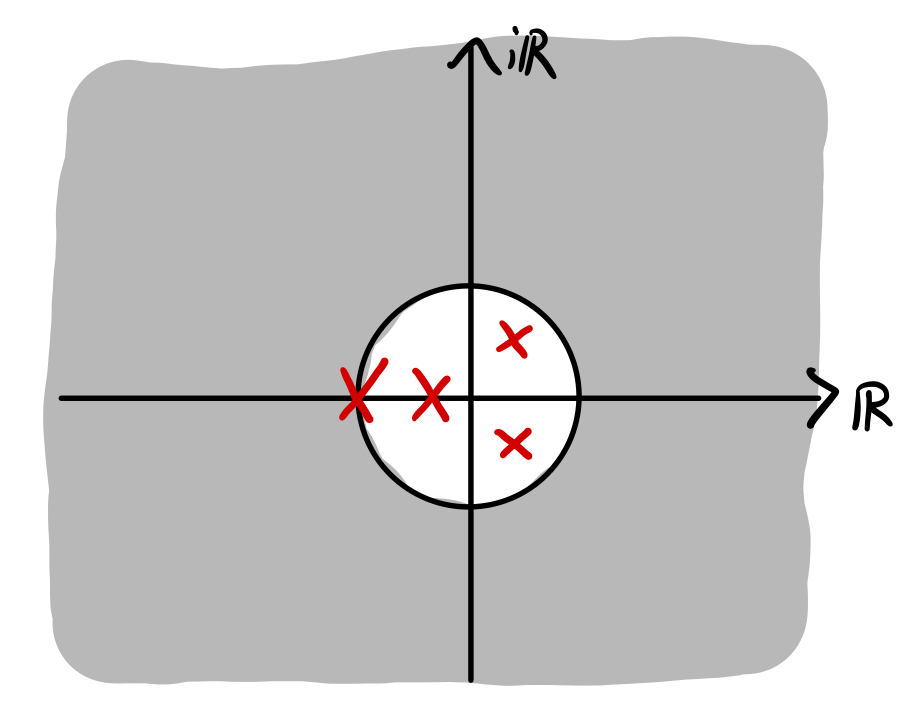
\includegraphics[width=0.3\linewidth]{docimgs/kausal.jpg}
\end{center}

\vspace*{-0.5cm}
\subsubsection*{BIBO-Stabilität}
\vspace*{-0.5cm}
$$\sum_{n=-\infty}^\infty |h[n]| < \infty \Leftrightarrow \sum_{n=-\infty}^\infty |h[n]z^{-n}| < \infty \text{ mit } |z|=1$$
Das heisst, das LTI-System ist BIBO-stabil, falls der \textbf{Einheitskreis in der ROC}$_H$ liegt, d.h. wenn $\{ z \in \mathbb{C} \; : \; |z| = 1 \} \subseteq \text{ROC}_H$. Wenn $H(z)$ rational ist, ist es eine Äquivalenz.

\vspace*{-0.5cm}
\begin{center}
    \begin{minipage}[c]{0.3\textwidth}
        \begin{flushright}
            \textbf{Beidseitig}
        \end{flushright}
    \end{minipage}
    \hfill
    \begin{minipage}[c]{0.25\textwidth}
        \begin{center}
            \textbf{Rechtsseitig}
        \end{center}
    \end{minipage}
    \hfill
    \begin{minipage}[c]{0.3\textwidth}
        \begin{flushleft}
            \textbf{Linksseitig}
        \end{flushleft}
    \end{minipage}
    
    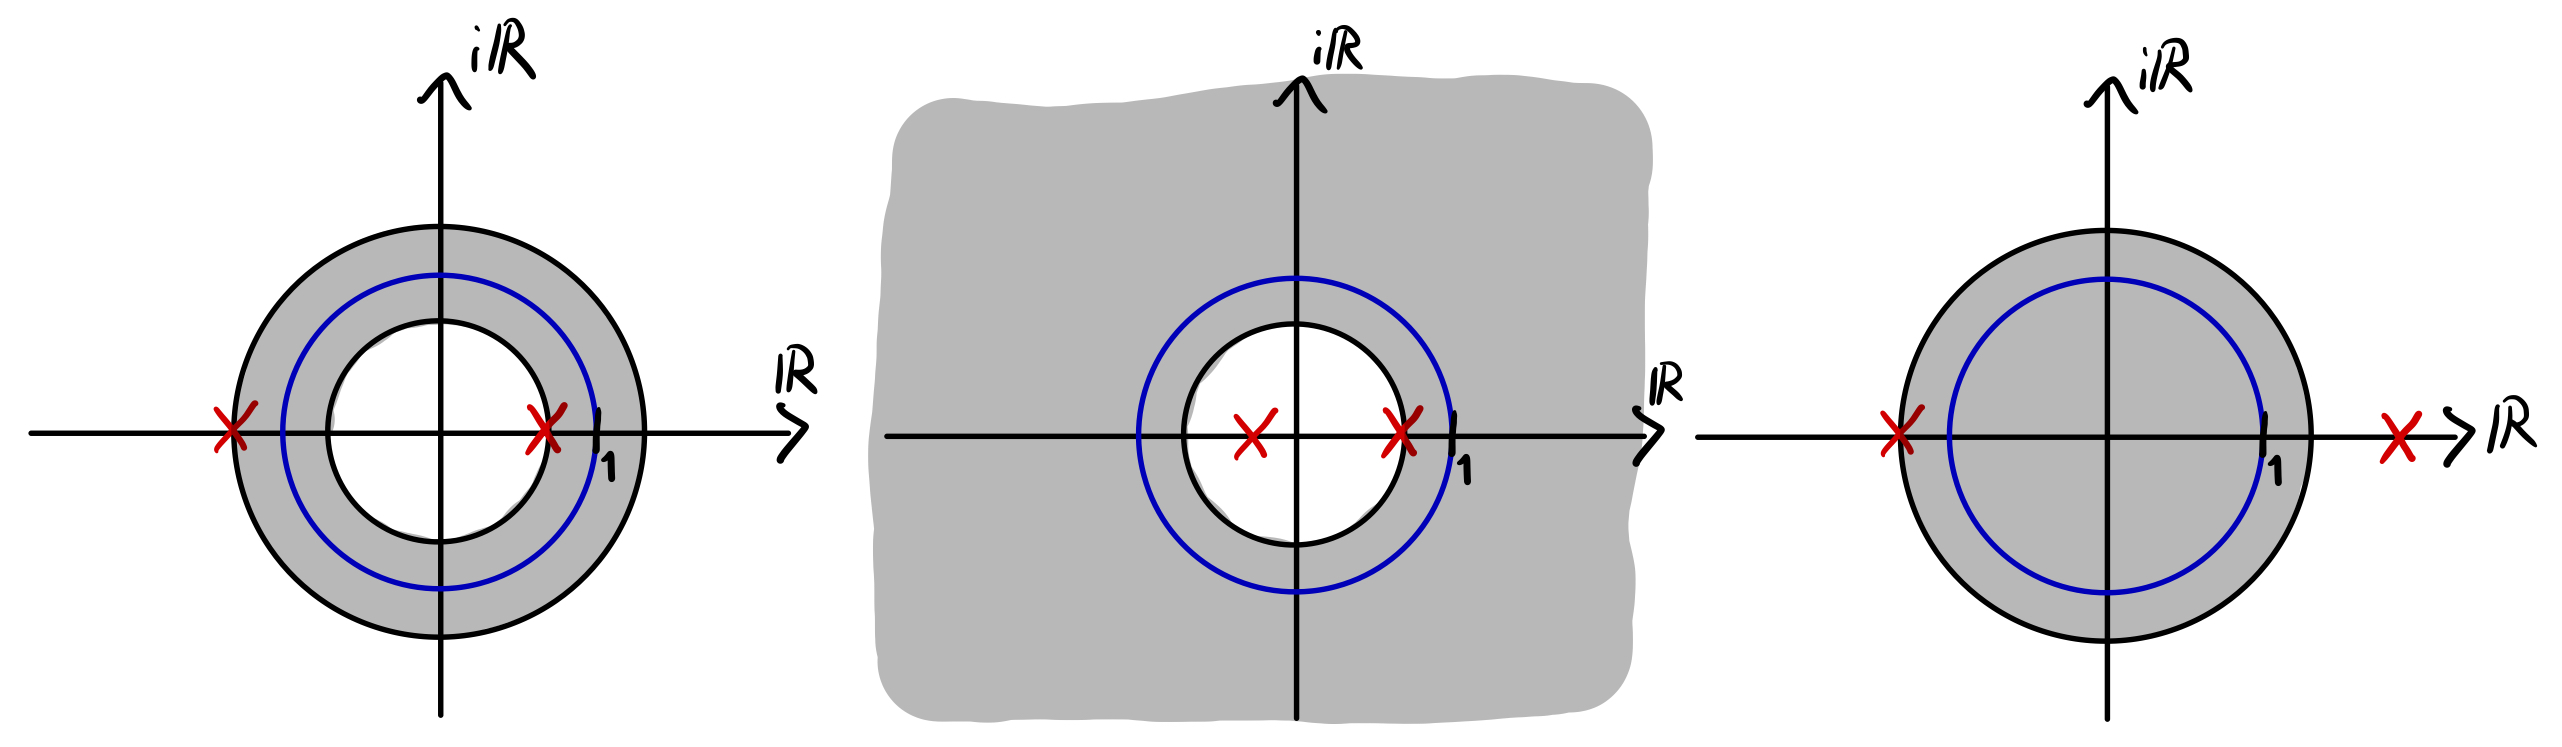
\includegraphics[width=0.8\linewidth]{docimgs/BIBO_stabil.jpg}
\end{center}

\pagebreak

\subsection*{Zusammenschaltung von LTI-Systemen}
\begin{enumerate}
    \item \textbf{Serienschaltung}:
    \item[] \noindent
            \begin{minipage}[t]{0.45\textwidth}
            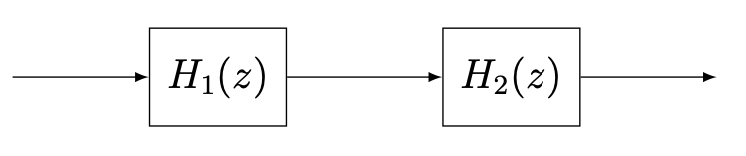
\includegraphics[width=\linewidth]{docimgs/Serienschaltung.png}
            \end{minipage}
            \hfill
            \begin{minipage}[c]{0.45\textwidth}
            $$H(z) = H_1(z)H_2(z)$$
            \vspace*{0.77cm}
            \end{minipage}
    \vspace*{-1cm}
    \item \textbf{Parallelschaltung}:
    \item[] \noindent
            \begin{minipage}[t]{0.45\textwidth}
            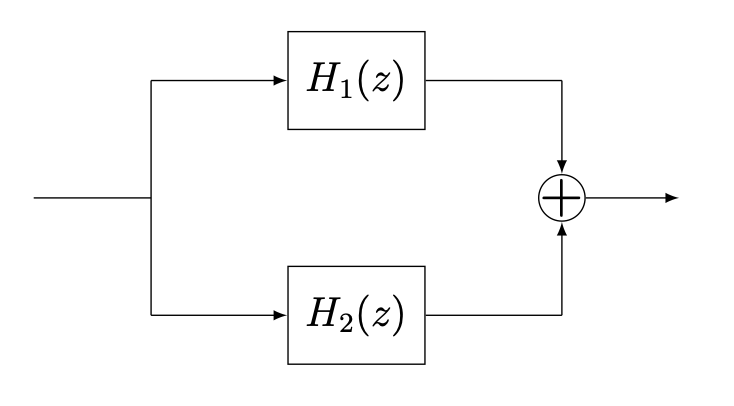
\includegraphics[width=\linewidth]{docimgs/Parallelschaltung.png}
            \end{minipage}
            \hfill
            \begin{minipage}[c]{0.45\textwidth}
            $$H(z) = H_1(z) + H_2(z)$$
            \vspace*{3.45cm}
            \end{minipage}
    \vspace*{-2.35cm}
    \item \textbf{Rückkopplung}:
    \item[] \begin{minipage}[t]{0.45\textwidth}
            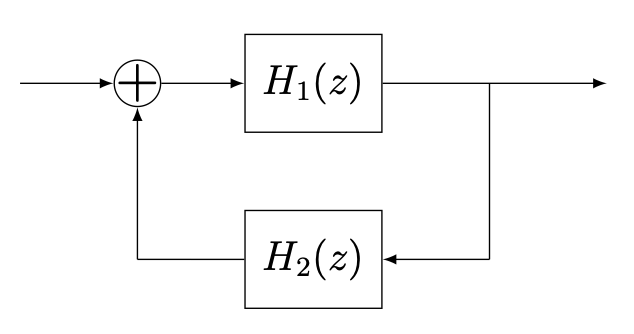
\includegraphics[width=\linewidth]{docimgs/Rueckkopplung.png}
            \end{minipage}
            \hfill
            \begin{minipage}[c]{0.45\textwidth}
            \begin{align*}
                &X(z)H_1(z) + H_2(z)Y(z)H_1(z) = Y(z) \\
                &X(z)H_1(z) = Y(z)(1-H_1(z)H_2(z)) \\
                &H(z)=\frac{H_1(z)}{1-H_1(z)H_2(z)}
            \end{align*}
            \vspace*{3.45cm}
            \end{minipage}
\end{enumerate}

\vfill \null
\pagebreak

\subsection*{Prüfungsaufgabe: Frühjahr 2023, Aufgabe 3}
\vspace*{-0.5cm}
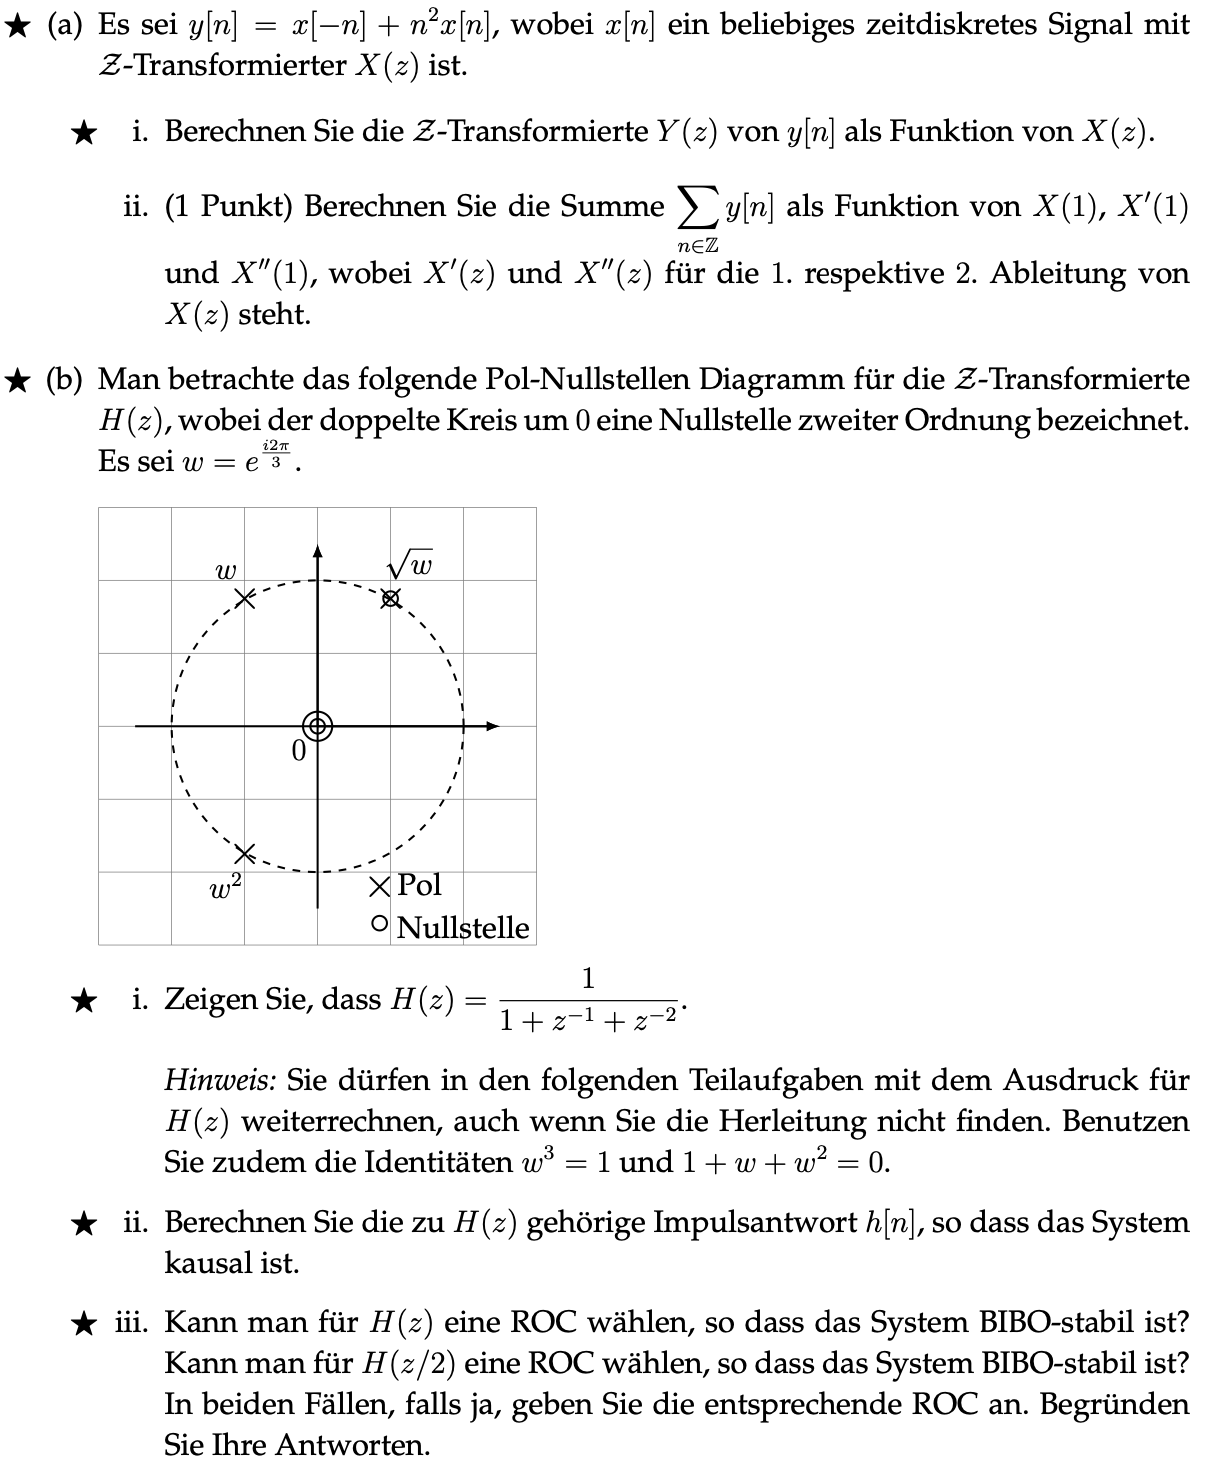
\includegraphics[width=0.9\linewidth]{docimgs/23ab.png}

\pagebreak

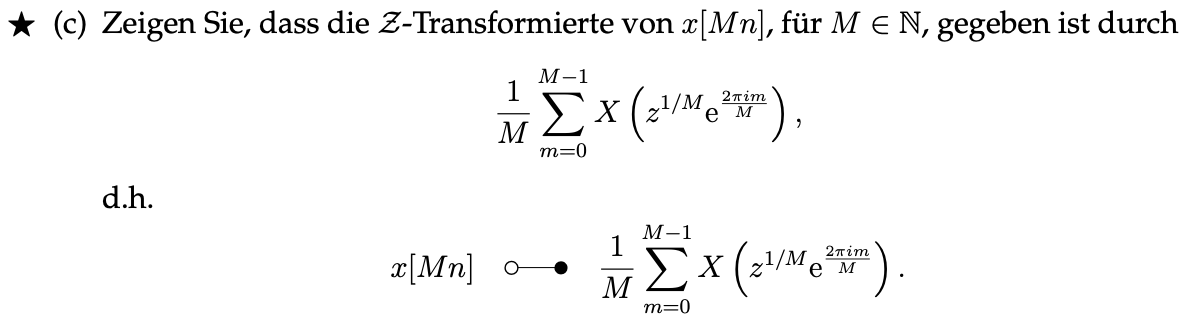
\includegraphics[width=0.9\linewidth]{docimgs/23c.png}


\begin{tikzpicture}
    % Define the box size and grid spacing
    \draw[step=0.5cm,gray!50,very thin] (0,0) grid (16.5,16
    ); % (0,0) is bottom-left corner, (10,10) is top-right corner
\end{tikzpicture}

\pagebreak


\begin{tikzpicture}
    % Define the box size and grid spacing
    \draw[step=0.5cm,gray!50,very thin] (0,0) grid (16.5,21
    ); % (0,0) is bottom-left corner, (10,10) is top-right corner
\end{tikzpicture}


\end{document}